\documentclass[submit,techrep]{ipsj}
% \documentclass{ipsj}

\usepackage{graphicx}
\usepackage{latexsym}

\def\Underline{\setbox0\hbox\bgroup\let\\\endUnderline}
\def\endUnderline{\vphantom{y}\egroup\smash{\underline{\box0}}\\}
\def\|{\verb|}

\setcounter{巻数}{59}
\setcounter{号数}{1}
\setcounter{page}{1}

% \受付{2016}{3}{4}
% \再受付{2015}{7}{16}   %省略可能
% \再再受付{2015}{7}{20} %省略可能
% \再再受付{2015}{11}{20} %省略可能
% \採録{2016}{8}{1}

\begin{document}


\title{アプリ開発における異なる実践共同体の\\
可視化システムの開発}

\etitle{Development of visualization system of different community of practice in application development}

\paffiliate{Arcana}{株式会社スタジオ・アルカナ\\
Studio Arcana, Inc.}

\paffiliate{Meisei}{明星大学情報学研究科情報学専攻\\
Department of Computer Science, Graduate School of Systems and Information Engineering, Meisei University}

\author{遠藤 勝也}{Katsuya Endoh}{Arcana}[k.endo@s-arcana.co.jp]
\author{武富 拓也}{Takuya Taketomi}{Meisei}
\author{尼岡 利崇}{Toshitaka Amaoka}{Meisei}

\begin{abstract}
本研究では,アプリケーション開発における異なる実践共同体の参加の過程を可視化するシステムを開発した.
著者らは過去に質的アプローチの観点から実践共同体(Community of Practice以下,CoP)の概念を用いて,異なる背景を持つプロジェクトメンバーの関係のあり方が,開発されるアプリケーションにどのような影響を及ぼすかという研究を行った.その研究結果をもとにCSCW(Computer Supported Cooperative Work)の観点から,アプリケーション開発の過程における,背景の異なるプロジェクトメンバーの関わり方を可視化するシステムの開発を行った.本システムを使用することにより,異なる背景を持つメンバーが参加するアプリ開発チームにおいて,アプリのデザインをメンバー間の関係構築のあり方からデザインを考えることを支援することを目的としている.
\end{abstract}


\begin{jkeyword}
実戦共同体,CSCW,PBL,情報可視化
\end{jkeyword}

\begin{eabstract}
In this study, we have developed a system that visualizes the process of participation of different community of practice in application development.
In the past, the authors used the concept of Community of Practice (CoP) from the perspective of a qualitative approach, and how the relationships between project members with different backgrounds affect the applications being developed. I did a study. Based on the research results, we developed a system that visualizes the involvement of project members with different backgrounds in the process of application development from the viewpoint of CSCW (Computer Supported Cooperative Work). By using this system, the purpose is to support the design of the application from the way of building relationships between the members in the application development team in which members with different backgrounds participate.
\end{eabstract}

\begin{ekeyword}
Community of Practice, CSCW, PBL, Data Visualization
\end{ekeyword}

\maketitle

%1
\section{はじめに}

グローバル化のもとで社会は複雑化し,ICTの進歩はめざましく,様々な業種や分野でソフトウェア・アプリケーションがなくてはならないものとなっている.現在のソフトウェア・アプリケーション(以下,アプリ)の開発は,プログラマーのみで完結することは少なく,多様な背景を持つメンバーと協働で開発が行われる.また共同開発では様々なICTツールが導入され,アプリの開発環境それ自体も変化している.


本研究は,過去に行った異なる背景を持つプロジェクトメンバーの関係構築のあり方が,開発されるアプリケーションのデザインにどのような影響を及ぼすかという研究の結果に基に行われたものである.過去研究は大学の専門分野横断型PBL(Project based learning)を対象として行われており,その結果をもとにCSCW(Computer Supported Cooperative Work)の観点からアプリケーション開発の過程における,背景の異なるプロジェクトメンバーの関わり方を可視化するシステムの開発を行った.


開発したシステムは,アプリ開発支援システムとして,ソフトウェアの開発手法の一つであるアジャイル開発に活用されることを目的としている.アジャイル開発とは機能単位の小さなサイクルで,設計・開 発・テストの工程を繰り返すことにより,様々な状況の変化に対応しながら開発を進めていく手法である.状況の変化に対応するため,日毎にdaily scrumと呼ばれる短い時間での進捗の 共有と反省を行う打ち合わせの時間が設けられている.[?]導入するアプリ開発支援ソフトウェアはdaily scrumに活用されることが想定されている.
アプリ開発支援ソフトウェアを利用することで,アプリを開発するプロジェクトメンバーは,アプリの要件を機能中心で考えるのではなく,プロジェクトメンバーの関係性からも把握できるようになる.結果的に,開発されるアプリの機能やUIは,技術や機能中心に決定されるのではなく,プロジェクトメンバーが持つリソースを十分に利用できるような関係性から考えられるようになることを想定している.

%2
\section{先行研究}
\label{previous-research}

本研究は,道具やテクノロジーの開発によって人々の協調的作業を支援するシステムの開発を目標としたCSCWの観点から[?],アプリケーション開発における異なる実践共同体の参加の過程を可視化するシステムを開発したものである.CSCWの発展はエスノメソドロジーに依拠したL.サッチマンの影響を大きく受けている言える.サッチマンは人々が社会生活を営むために用いる「やり方」[?]を分析することを目的をするエスノメソドロジーの手法により,人間の行動は状況依存的に組織されていることを主張した[?].このような社会の行為を状況との関わりの中で分析する研究は,サッチマン以外にもE.ウェンガーが主張する実践共同体[?]の理論や,日本では,上野直樹を中心とした状況論の研究が行われている[?].

CSCWへの研究の発展に大きな貢献をしたサッチマンであったが,同時に異分野横断的研究について,組織上の困難さを抱えていた[?].その苦悩とは,異なる専門性にかかわる分業的な関係のあり方,つまり,情報学研究とエスノメソドロジーの知識産出のプロセスや前提とする認識論のズレも関係していたと考えられる[?].このような異なる背景を有するコミュニティのメンバー同士がコミュニケーションを行う場合,異分野横断的研究に関わらず,企業の部門間でも認識論の違いから主張の食い違いや対立が起きることもある[?].

上記のような異なる専門性や背景をもつメンバー同士の関係についてどのように実践が行われているかの分析を行うには,実践共同体の概念を用いることが有効であると考える.
実践共同体とは,成員の学習の促進あるいは知識を共有・創造といったある一定のテーマや目的のもとに構築された共同体である[?].実践共同体には,正統的周辺参加,ディスコース,布置といった概念を含んでいる.正統的周辺参加とは,成員がある実践共同体に加わり,技能の獲得と成員のアイデンティティの発達を達成していくその軌跡(Trajectory)を表す概念である.ディスコースとは,実践共同体に共有される話し手のミクロな会話からマクロな価値観まで含む文化のことを意味する.布置とは,成員は単一の実践共同体のみに参加するものではなく,複数の実践共同体の参加することから,複数の実践共同体に参加しその関係を捉える概念である.

実践共同体の概念を用いた研究について,学習という側面に関し ての多くの研究で効果が指摘されているが,異なるCoPの関係構築のあり方と開発されるアプリへの影響と変化を扱う研究は著者が知る限り少ない.しかし,上野[2]が示すように人工物は,様々な組織間やコミュニティ間の調停,交渉の産物として形成されており,人工物のデザインとはコミュニティのデザインであると述べているように,実践共同体の概念を用いた分析は学習以外にも焦点を向ける有用性があると考えられる.そのため,異なる背景を持つメンバー同士の関係のあり方を実践共同体の概念から分析し,生み出される人工物のデザインー本研究ではアプリのデザインーを紐付けるプロセスは有効であると考える.


人文学部国際関係学科(以下,学科)と情報学部情報学科は,目的とする専門性や実践の違いから異なるCoPであると考えられる.研究対象のプロジェクト授業に参 加する国コミ学科の学生は英語でのプレゼンテーションが主な実践であり,情報学科の学生は プログラミングやアプリ開発が主な実践となる.  アプリ開発のプロセスにおいて,当然ながらアプリの実装が完了した後で,英語でのプレゼ ンテーションという順番になるため,両学科の学生が積極的に参加するタイミングは時期によって齟齬がおきる.加えて,国コミ学科はアプリ開発に携わった経験があるものはまれなた め,プロジェクト前半ではアプリ開発におけるコミュニケーションは積極的に意見を出すというよりも,観察を主とした参加の態度になる.これはCoPでいう正当的周辺参加と言い換えることができる.他方,情報学科は技術それ自体が主な実践のため,成果発表よりも技術のそれ 自体に価値を見出す傾向が見られる.  上記のように,両学科の学生が重きを置く実践(あるいは専門)の違いが,プロジェクトに積 極的に参加する時期のずれを生み出す.その結果,言葉の解釈の違い,プロジェクトにおける時間感覚のずれなどのディスコミュニケーションを引き起こす.  またプロジェクトに参加する態度として,自分の専門性に関わるタスクしか関心を向けない という態度は分業的なタスクの割り振りを引き起こし,このこともまたディスコミュニケー ションを引き起こす原因となる.他方,自分の専門を超えて,両学科が一緒に作業をする時間を設けることで,アプリ開発の過程やプレゼンテーション資料作成の過程に協働で関与する中 で,言葉の意味の交渉や目的の共有が行われ,人工物のデザインに異なる専門の知識や技術的なリソースが影響する.これはCoPでいう布置として扱われる.上記のように分業的,あるいは協働的といった関係のあり方がそれ自体が人工物の機能やUIに影響を及ぼすのではないかと いう示唆を得ている.


本研究が対象とする授業は,両学科が自ら主とする実践や専門を越えて協働で作業すること により,お互いの実践を融合させてプロジェクトの目的を達成するように授業構成が行われて いる.そのため,本研究で導入するアプリ開発ソフトウェアは,アプリ開発の要件から実装ま でを機能中心に組み立てるのではなく、参加者それぞれの関心やスタンスを調整しその関係の あり方そのものからデザインすることを目的として実装されている.


 アプリ開発支援ソフトウェアは,Atlassia社が提供するプロジェクトのタスク管理をするた めのオンラインツールである「Trello」と連携して開発されたものである.Trelloが提供する API(Application Programming Interface)を使用して,Trelloのタスクが持つデータを抽出 し,グラフ構造として可視化する.この可視化機能により分業的,あるいは協働的にタスクを こなしているかを確認しながら,アプリ開発を行えるような想定をしている(図1).アプリ開 発支援ソフトウェアは,CoPの概念を参考に設計されており,「正統的周辺参加」をTrelloの カードの移動,プロジェクトのタスクがどの共同体に属しいてるかをTrelloのラベル機能を用 いて表す.


\section{本システムについて}
\label{system-map}

本システムでは,
プロジェクトメンバーをノード,
プロジェクトメンバーが共同でタスクを行った履歴をエッジとした,
ネットワーク構造でプロジェクトメンバーの関係性を可視化している.
本システムによって可視化したプロジェクトメンバーの関係性を,
図\ref{cop-map-graph}に示す.

本システムでは,ネットワーク構造のレイアウト手法として,力学モデルを採用している.
その際に,共同作業を行った回数によってエッジの強度を変化させるている.
よって,多くのタスクを共同で行うほど,
ノード間の距離は近くなるように配置される.
% これにより,

また,プロジェクトメンバーの所属先によってノードの色を変化させることで,
異なるCoPに所属するプロジェクトメンバーの共同作業を観察することを可能にしている.
これにより,異なる色のノードがエッジでつながっている様子から,
布置を観察することを可能にしている.

さらに,タスクを行った回数の合計値によってノードの大きさを変化させる.
これにより,ノードの大きさは小さいが,他のノードとの繋がりがみられる場合に,
そのプロジェクトメンバーは正統的周辺参加であるという可能性を観察することができる.

以上のネットワーク構造を,プロジェクトの時系列順に変化させることで,
プロジェクトメンバーの関係性の変化を観察することを可能にしている.
これにより,ノードの軌跡から,
進行状況によって変化していく,
プロジェクトメンバーの軌跡を観察することを可能にしている.

% \begin{enumerate}
%    \item CoP
%    \item 布置
%    \item トラジェクトリー
%    \item 正統的周辺参加
% \end{enumerate}

\begin{figure}[h]
  \centering
  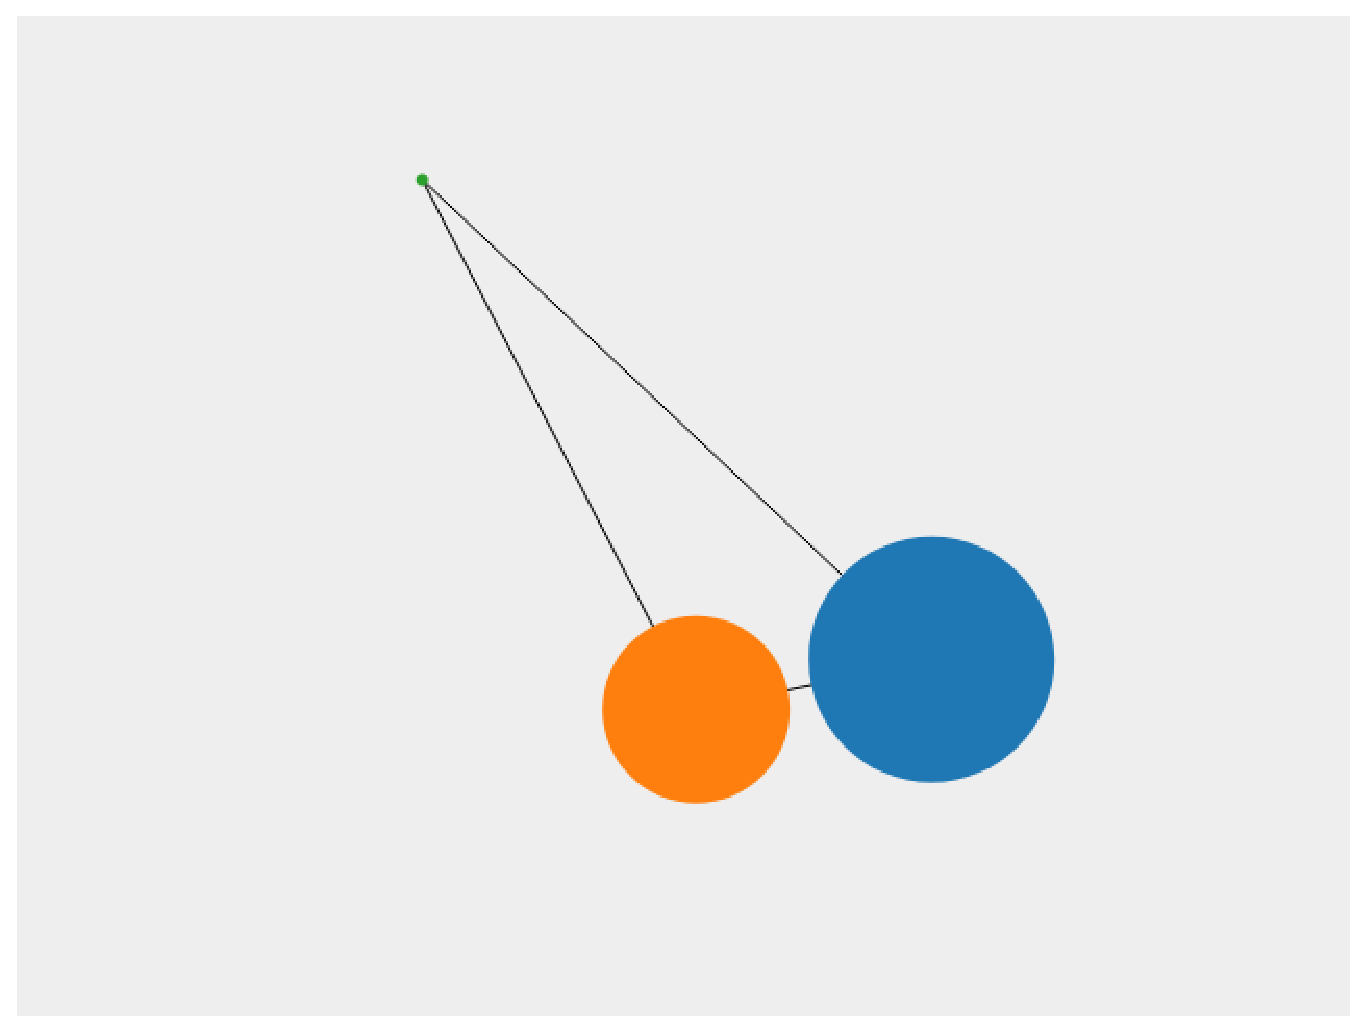
\includegraphics[width=0.5\textwidth]{img/cop-map-graph.eps}
  \caption{本システムによってプロジェクトメンバーの関係性を可視化した様子}
  \label{cop-map-graph}
\end{figure}

% 本システムは,アプリケーションサーバとデータベース,
% 外部サービスであるTrelloから構成されている.
%
% タスクの履歴を,TrelloのWeb APIから取得して,
% 時系列順にネットワーク構造に整形することで可視化している.

%4
\section{今後の展望}

%5
\section{おわりに}

\begin{thebibliography}{9}
\bibitem{okumura}
奥村晴彦:改訂第5版 \LaTeXe 美文書作成入門,
技術評論社(2010).

\bibitem{companion}
Goossens, M., Mittelbach, F. and Samarin, A.: {\it The LaTeX Companion},
Addison Wesley, Reading, Massachusetts (1993).

\bibitem{book1}
木下是雄:
理科系の作文技術,
中公新書(1981).

\bibitem{book2}
Strunk, W.J. and White, E.B.: {\it The Elements of Style, Forth Edition},
Longman (2000).

\bibitem{book3}
Blake, G. and Bly, R.W.: {\it The Elements of Technical Writing},
Longman (1993).

\bibitem{book4}
Higham, N.J.:
{\it Handbook of Writing for the Mathematical Sciences},
SIAM (1998).

\bibitem{webpage1}
情報処理学会論文誌ジャーナル編集委員会:
投稿者マニュアル(オンライン),
\urlj{http://www.ipsj.or.jp/journal/ submit/manual/j\_manual.html}%
\refdatej{2007-04-05}.

\bibitem{webpage2}
情報処理学会論文誌ジャーナル編集委員会:
べからず集(オンライン),
\urlj{http://www.ipsj.or.jp/journal/\\ manual/bekarazu.html}%
\refdatej{2011-09-15}.

\end{thebibliography}

\begin{biography}
\profile{n}{遠藤 勝也}{1992年生.2016年明星大学情報学部情報学科卒業.
2018年株式会社スタジオ・アルカナ入社.ウェブサービス開発に従事.芸術科学会会員.}
%
\profile{n}{武富 拓也}{1990年生.2016年明星大学人文部国際コミュニケーション学科卒業.
2019年明星大学情報学部実習指導員として勤務, 明星大学大学院情報学研究科情報学専攻博士前期課程(研究生). 社会言語科学会会員}
%
\profile{h,L}{学会 次郎}{1950年生.1974年架空大学大学院修士課程修了.
1987年同博士課程修了.工学博士.1977年架空大学助手.1992年情報処理大学助
教授.1987年同大教授.2000年から情報処理学会顧問.オンライン出版の研究
に従事.2010年情報処理記念賞受賞.情報処理学会理事.電子情報通信学会,
IEEE,IEEE-CS,ACM 各会員.}
\end{biography}

\end{document}
